\documentclass[12pt]{article}
\usepackage{setspace}
\doublespacing
\usepackage{times}
\usepackage{natbib}
\usepackage{fullpage}
\usepackage{tikz}
\usepackage{amsmath,amssymb}
\usepackage{hyperref}
\usepackage{graphicx}
\usepackage{algorithmic}
\usepackage{multirow}

\DeclareMathOperator*{\argmin}{arg\,min}
\DeclareMathOperator*{\Lik}{Lik}
\DeclareMathOperator*{\PoissonLoss}{PoissonLoss}
\DeclareMathOperator*{\Peaks}{Peaks}
\DeclareMathOperator*{\Segments}{Segments}
\DeclareMathOperator*{\argmax}{arg\,max}
\DeclareMathOperator*{\maximize}{maximize}
\DeclareMathOperator*{\minimize}{minimize}
\newcommand{\sign}{\operatorname{sign}}
\newcommand{\keyword}[1]{\textbf{#1}}
\newcommand{\RR}{\mathbb R}
\newcommand{\ZZ}{\mathbb Z}
\newcommand{\NN}{\mathbb N}

\begin{document}

\title{Introduction to machine learning and neural networks}

\author{
  Toby Dylan Hocking\\
  toby.hocking@nau.edu
}

\maketitle


% Your manuscript is 20 or fewer pages, double space, including figures and tables, for each lecture or practice. That makes about 10 book pages. Exception is possible for a few lectures.

% Each manuscript may include 3-5 illustrations.

% Manuscript should be written at a level to be understood by first-year graduate students. 

% Each manuscript has a short, first paragraph (<50 words) about the training goal.

% Do not have too many references as it is not a research paper but list a few suggested readings.

% Include a few (4-6) quizzes for each lecture and expected homework for each practice.

% Text in your chapter should be corresponding to the pre-recorded video or the video to be recorded.

\paragraph{Objective.} This chapter introduces basic concepts and
algorithms from machine learning. The goal is to learn how to use
cross-validation for training and testing machine learning algorithms,
and to implement neural networks in R code.

\section{Introduction and applications of machine learning}

Machine learning is the domain of computer science which is concerned
with efficient algorithms for making predictions in all kinds of big
data sets. A defining characteristic of supervised machine learning
algorithms is that they require a data set for training. The machine
learning algorithm then memorizes the patterns present in those
training data, with the goal of accurately predicting similar patterns
in new test data. Many machine learning algorithms are
domain-agnostic, which means they have been shown to provide highly
accurate predictions in a wide variety of application domains
(computer vision, speech recognition, automatic translation, biology,
medicine, climate science, chemistry, geology, etc). 

\begin{figure} 
  \centering
  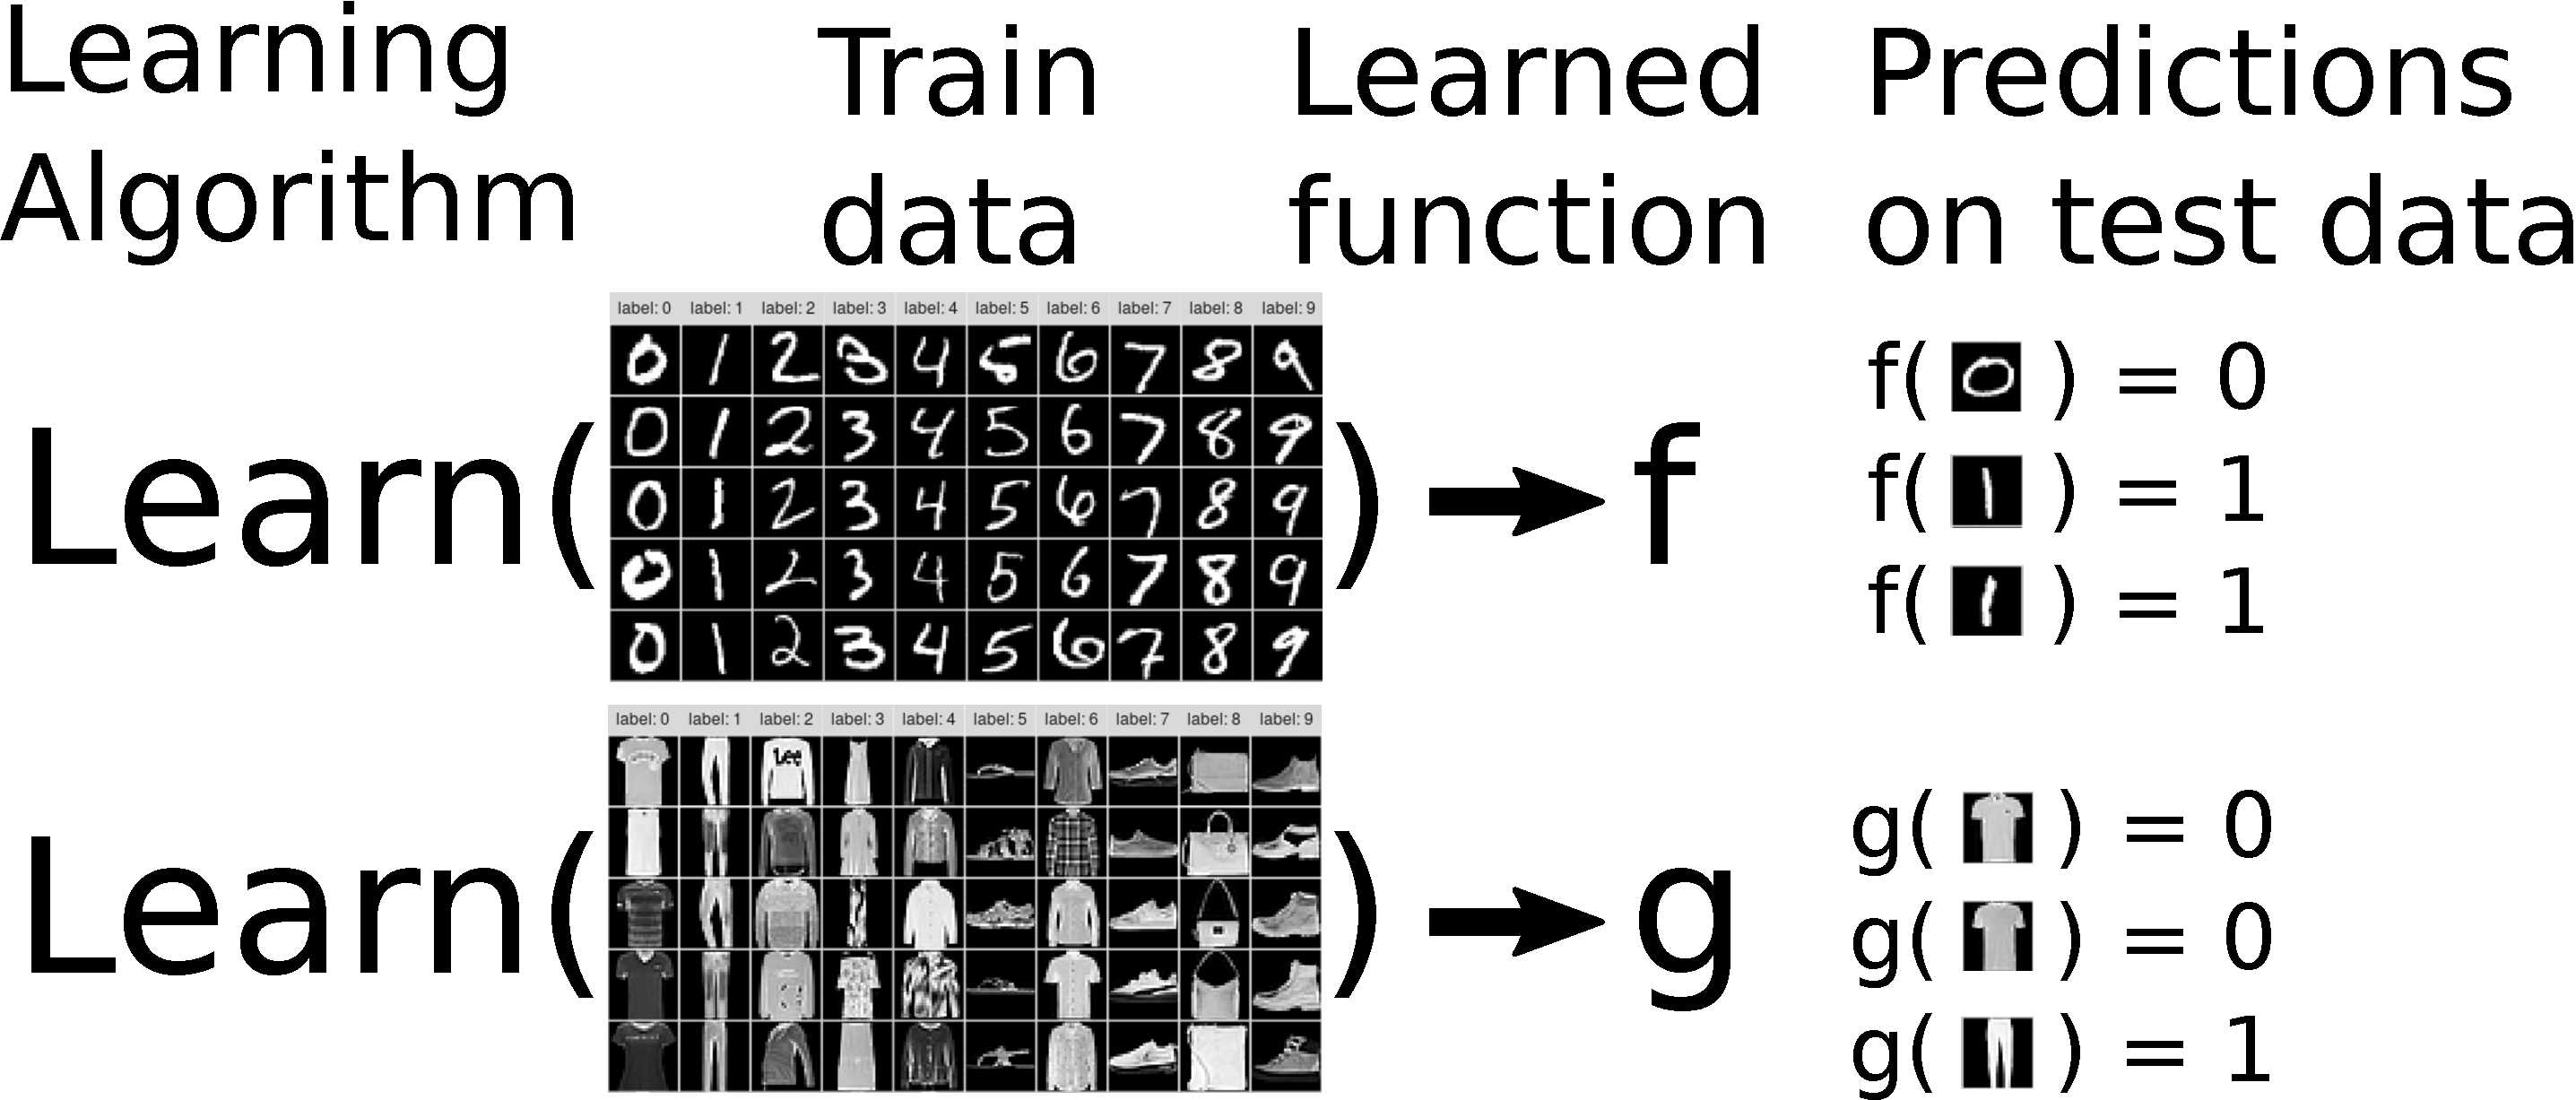
\includegraphics[width=0.8\textwidth]{drawing-mnist-train-test.pdf}
  \caption{A learning algorithm inputs a train data set, and outputs a
    prediction function, g or h. Both g and h input a grayscale image
    and output a class (integer from 0 to 9), but g is for  
    digits and h is for fashion.}
  \label{fig:drawing-mnist-train-test}
\end{figure}

For example, consider the problem of image classification from the
application domain of computer vision. In this problem, we would like
a function that can input an image, and output an integer which
indicates class membership. More precisely, let us consider the MNIST
and Fashion-MNIST data sets
(Figure~\ref{fig:drawing-mnist-train-test}), in which each input is
grayscale image with height and width of 28 pixels
\citep{LeCun1998,Xiao2017} then we typically represent each input as a
matrix of real numbers $\mathbf x\in\mathbb R^{28\times 28}$. In both
the MNIST and Fashion-MNIST data sets each image has a corresponding
label which is an integer $y\in\{0,1,\dots,9\}$. In the MNIST data set
each image/label represents a digit, whereas in Fashion-MNIST each
image/label represents a category of clothing (0 for T-shirt/top, 1
for Trouser, 2 for Pullover, etc).  In both data sets the goal is to
learn a function
$f:\mathbb R^{28\times 28}\rightarrow \{0,1,\dots, 9\}$ which inputs
an image $\mathbf x$ and outputs a predicted class $f(\mathbf x)$
which should ideally be the same as the corresponding label $y$.

As mentioned above, a big advantage of supervised learning algorithms
is that they are typically domain-agnostic, meaning that they can
learn accurate prediction functions $f$ using data sets with different
kinds of patterns. That means we can use a single learning algorithm
\textsc{Learn} on both the MNIST or Fashion-MNIST data sets
(Figure~\ref{fig:drawing-mnist-train-test}, left). For the MNIST data
set the learning algorithm will output a function for predicting the
class of digit images, and for Fashion-MNIST the learning algorithm
will output a function for predicting the class of a clothing image
(Figure~\ref{fig:drawing-mnist-train-test}, right). The advantage of
this supervised machine learning approach to image classification is
that the programmer does not need any domain-specific knowledge about
the expected pattern (e.g., shape of each digit, appearance of each
clothing type). Instead, we assume there is a data set with enough
labels for the learning algorithm to accurately infer the
domain-specific pattern and prediction function. This means that the
machine learning approach is only appropriate when it is
possible/inexpensive to create a large labeled data set that
accurately represents the pattern/function to be learned.

How do we know if the learning algorithm is working properly? The goal
of supervised learning is \keyword{generalization}, which means the
learned prediction function $f$ should accurately predict
$f(\mathbf x) = y$ for any inputs/outputs $(\mathbf x,y)$ that will be
seen in a desired application (including new data that were not seen
during learning). To formalize this idea, and to compute quantitative
evaluation metrics (accuracy/error rates), we need a test data set, as
explained in the next section.

\subsection{$K$-fold cross-validation for evaluating prediction/test accuracy}

Each input $\mathbf x$ in a data set is typically represented as one
of $N$ rows in a design matrix with $D$ columns (one for each
dimension or feature). Each output $y$ is represented as an element of
a label vector of size $N$, which can be visualized as another column
alongside the design matrix (Figure~\ref{fig:cross-validation},
left). For example, in the image data sets discussed above we have
$N=60,000$ labeled images/rows, each with $D=784$ dimensions/features
(one for each of the $28\times 28$ pixels in the image).

The goal of supervised learning is to find a prediction function $f$
such that $f(\mathbf x) = y$ for all inputs/outputs $(\mathbf x,y)$ in
a test data set (which is not available for learning
$f$). So how do we learn $f$ for accurate prediction on a test data
set, if that test set is not available? We must assume that we have
access to a train data set with the same statistical distribution as
the test data. The train data set is used to learn $f$, and the test
data can only be used for evaluating the prediction accuracy/error of
$f$.

Some benchmark data sets which are used for machine learning research,
like MNIST and Fashion-MNIST, have designated train/test
sets. However, in most applications of machine learning to real data
sets, train/test sets must be created. One approach is to create a
single train/test split by randomly assigning a set to each of the $N$
rows/observations, say 50\% train rows and 50\% test rows. The
advantage of that approach is simplicity, but the drawback is that we
can only report accuracy/error metrics with respect to one test set
(e.g., the algorithm learned a function which accurately predicted
91.3\% of observations/labels in the test set, meaning 8.7\% error
rate). 

In addition to estimating the accuracy/error rate, is important to
have some estimate of variance in order to make statements about
whether the prediction accuracy/error of the learned function $f$ is
significantly larger/smaller than other prediction functions. The
other functions to compare against may be from other supervised
learning algorithms, or some other method that does not use machine
learning (e.g., a domain-specific physical/mechanistic model). A common
baseline is the constant function $f(\mathbf x) = y_0$ where $y_0$ is
the average or most frequent label in the train data. This baseline
ignores all of the inputs/features $\mathbf x$, and can be used to
show that the algorithm is learning some non-trivial predictive relationship
between inputs and outputs (for an example see
Figure~\ref{fig:test-accuracy}).

\begin{figure}
  \centering
  \includegraphics[width=\textwidth]{drawing-cross-validation}
  \caption{$K=3$ fold cross-validation. \textbf{Left:} the first step
    is to randomly assign a fold ID from 1 to $K$ to each of the
    observations/rows. \textbf{Right:} in each of the
    $k\in\{1, \dots, K\}$ splits, the observations with fold ID $k$
    are set aside as a test set, and the other observations are used
    as a train set to learn a prediction function (f1--f3), which is
    used to predict for the test set, and to compute accuracy metrics
    (A1--A3).}
  \label{fig:cross-validation}
\end{figure}

The $K$-fold cross-validation procudure generates $K$ splits, and can
therefore be used to estimate both mean and variance of prediction
accuracy/error. The number of folds/splits $K$ is a user-defined
integer parameter which must be at least 2, and at most $N$. Typical
choices range from $K=3$ to 10, and usually the value of $K$ does not
have a large effect on the final estimated mean/variance of prediction
accuracy/error. The algorithm begins by randomly assigning a fold ID
number (integer from 1 to $K$) to each observation
(Figure~\ref{fig:cross-validation}, left). Then for each unique fold
value from 1 to $K$, we hold out the corresponding observations/rows
as a test set, and use data from all other folds as a train set
(Figure~\ref{fig:cross-validation}, right). Each train set is used to
learn a corresponding prediction function, which is then used to
predict on the held out test data. Finally, accuracy/error metrics are
computed in order to quantify how well the predictions fit the labels
for the test data. Overall for each data set and learning algorithm
the $K$-fold cross-validation procedure results in $K$ splits, $K$
learned functions, and $K$ test accuracy/error metrics, which are
typically combined by taking the mean and standard deviation (or
median and quartiles). Other algorithms may be used with the same fold
assignments, in order to compare algorithms in terms of accuracy/error
rates in particular data sets.

For example, Figure~\ref{fig:test-accuracy} uses $K=4$-fold
cross-validation to compare four learned functions on an image
classification problem. The accuracy rates of the ``dense'' and
``linear'' functions, $97.4 \pm 1.6 \%$ and $96.3 \pm 1.9 \%$ (mean
$\pm$ standard deviation) are not significantly different. Both rates
are significantly larger than the accuracy of the ``baseline''
constant function, $16.4 \pm 1.4 \%$, and smaller than the accuracy of
the ``conv'' function, $99.3 \pm 1.1 \%$. We can therefore conclude
that the most accurate learning algorithm for this problem, among
these four candidates, is the ``conv'' method (which uses a
convolutional neural network, explained later).  It is important to
note that statements about what algorithm is most accurate only makes
sense in terms of a particular data set, after having performed
$K$-fold cross-validation to estimate prediction accuracy/error rates.

\subsection{Other applications}

So far we have only discussed machine learning algorithms in the
context of a single prediction problem, image classification. In this
section we briefly discuss other applications of machine learning. In
each application the set of possible inputs $\mathbf x$ and outputs
$y$ are different, but machine learning algorithms can always be used
to learn a prediction function $f(x)\approx y$. 

\citep{Jones2009} proposed to use interactive machine learning for
cell image classification in the CellProfiler Analyst system. This
application is similar to the previously discussed digit/fashion
classification problem, but with only two classes (binary
classification). In this context the input is a multi-color image of
cell $\mathbf x\in\mathbb R^{h \times w \times c}$ where $h,w$ are the
height and width of the image in pixels, and $c=3$ is the number of
channels used to represent a color image (red, green, blue). The
output $y\in\{0,1\}$ is a binary label which indicates whether or not
the image contains the cell phenotype of interest. 

Some email programs use machine learning for spam filtering, which is
another example of a binary classification problem. When you click the
``spam'' button in the email program you are labeling that email as
spam ($y=1$), and when you respond to an email you are labeling that
email as not spam ($y=0$). The input $\mathbf x$ is an email message,
which can be represented using a ``bag-of-words'' vector (each element
is the number of times a specific word occurs in that email message).

\citet{Russell2008} proposed the LabelMe tool for creating data sets
for image segmentation, which is more complex than the previously
discussed image classification problems. In this context the input
$\mathbf x\in\mathbb R^{h \times w \times c}$ is typically a
multi-color image, and the output
$\mathbf y\in \{0,1\}^{h \times w}$ is a binary mask (one element
for every pixel in the image) indicating whether or not that pixel
contains an object of interest.

Machine learning can be used for automatic translation between
languages. In this context the input is a text in one language (e.g.,
French) and the output is the text translated to another language
(e.g., English). The desired prediction function $f$ inputs a French
text and outputs the English translation.

Machine learning can be used for medical diagnosis. For example
\citet{Poplin2017} showed that retinal photographs can be used to
predict blood pressure or risk of heart attack. Since the output $y$
is a real number (e.g., blood pressure of 120 mm mercury), we refer to
this as a regression problem.

\section{Avoiding under/overfitting in a neural network for regression}

Now we consider a simple regression problem for which the input
$x\in\mathbb R$ is a single real number ($D=1$ feature/column in the
design matrix), and the output $y\in\mathbb R$ is as well. Using a
neural network with a single hidden layer of $U$ units, there are two
unknown \keyword{parameter} vectors which need to be learned using the training
data, $\mathbf w\in \mathbb R^U$ and $\mathbf v\in \mathbb R^U$. The prediction
function $f$ is then defined as
\begin{equation}
  f(x) = \mathbf w^\intercal \sigma( x \mathbf v ) = \mathbf w^\intercal \mathbf z,
\end{equation}
where $\sigma:\mathbb R^U\rightarrow \mathbb R^U$ is a non-linear
activation function, and $\mathbf z\in \mathbb R^U$ is the vector of
hidden units. Typical activation functions include the logistic
sigmoid $\sigma(t)=1/(1+\exp(-t))$ and the rectifier (or rectified
linear units, ReLU) $\sigma(t)=\max(0, t)$. The prediction function is
learned using gradient descent, which is an algorithm that attempts to
find parameters $\mathbf w,\mathbf v$ which minimize the mean squared
error between the predictions and the corresponding labels in the $N$
train data,
\begin{equation}
  \mathcal L(\mathbf w, \mathbf v) = \frac{1}{N} \sum_{i=1}^N [ \mathbf w^\intercal \sigma( x_i \mathbf v ) - y_i ]^2. \label{eq:loss}
\end{equation}
Gradient descent begins using un-informative parameters
$\mathbf w_0,\mathbf v_0$ (typically random numbers close to zero),
then at each iteration $t\in\{1,\dots, T\}$ the parameters are
improved by taking a step of size $\alpha>0$ in the negative gradient
direction,
\begin{eqnarray}
  \mathbf w_t &=& \mathbf w_{t-1} - \alpha \nabla_{\mathbf w} \mathcal L(\mathbf w, \mathbf v),\\
  \mathbf v_t &=& \mathbf v_{t-1} - \alpha \nabla_{\mathbf v} \mathcal L(\mathbf w, \mathbf v).
\end{eqnarray}
The algorithm described above is referred to as ``full gradient''
because the gradient is defined using the full set of $N$ samples in
the train set. Other common variants include ``stochastic gradient''
(gradient uses one sample) and ``minibatch'' (gradient uses several
samples). When doing gradient descent on a neural network model, one
``epoch'' includes computing gradients once for each sample (e.g., 1
epoch = 1 iteration of full gradient, 1 epoch = $N$ iterations of
stochastic gradient).

In the algorithm above, the number of hidden units $U$, the number of
iterations $T$, and the step size $\alpha$ must be fixed before
running the learning algorithm. These \keyword{hyper-parameters}
affect the learning capacity of the neural network.  An important
consideration when using any machine learning algorithm is that you
most likely need to tune the hyper-parameters of the algorithm in
order to avoid underfitting and overfitting. \keyword{Underfitting}
occurs when the learned function $f$ neither provides accurate
predictions for the train data, nor the test
data. \keyword{Overfitting} occurs when the learned function $f$ only
provides accurate predictions for the train data (and not for the test
data). Both underfitting and overfitting are bad, and need to be
avoided, because the goal of any learning algorithm is to find a
prediction function $f$ which provides accurate predictions in test
data.

\begin{figure}
  \centering
  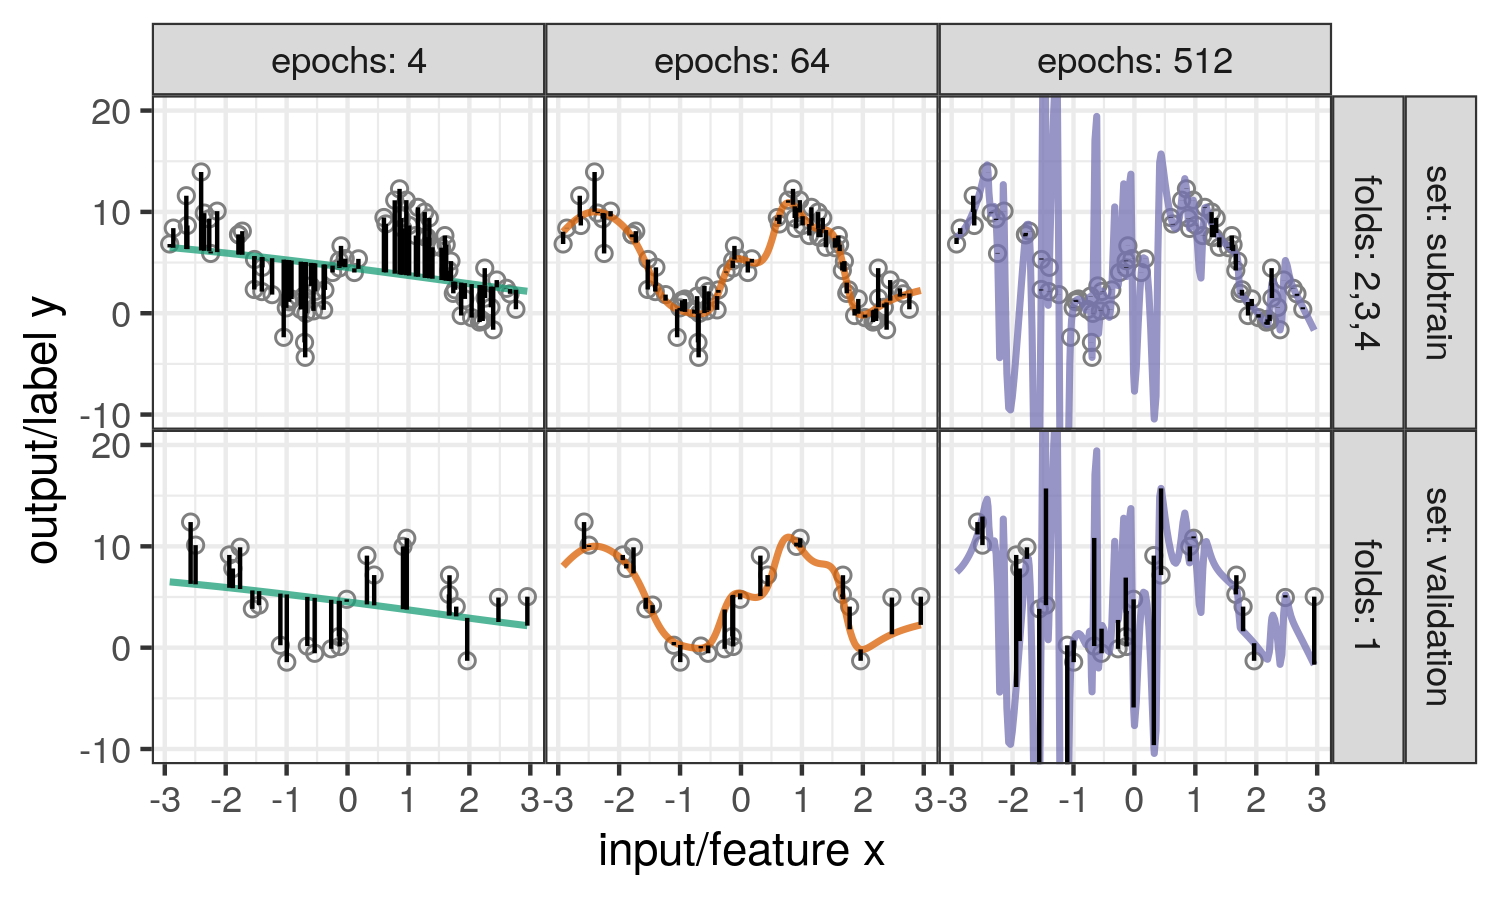
\includegraphics[width=0.55\textwidth]{figure-overfitting-paper}
  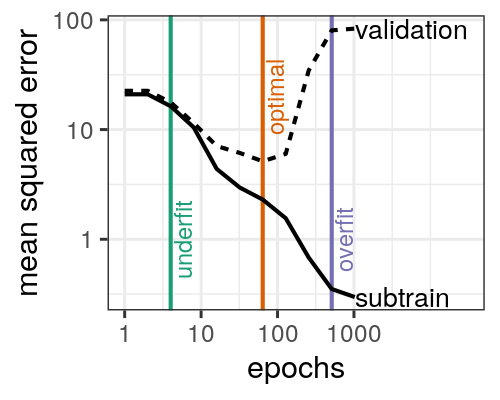
\includegraphics[width=0.4\textwidth]{figure-overfitting-paper-loss}   
  \caption{Illustration of underfitting and overfitting in a neural
    network regression model (single hidden layer, 50 hidden
    units). \textbf{Left:} noisy data with a nonlinear sine wave
    pattern (grey circles), learned functions (colored curves), and
    residuals/errors (black line segments) are shown for three values
    of epochs (panels from left to right) and two data subsets (panels
    from top to bottom). \textbf{Right:} in each epoch the model
    parameters are updated using gradient descent with respect to the
    subtrain loss, which decreases with more epochs. The
    optimal/minimum loss with respect to the validation set occurs at
    64 epochs, indicating underfitting for smaller epochs (green
    function, too regular/linear for both subtrain/validation sets)
    and overfitting for larger epochs (purple function, very
    irregular/nonlinear so good fit for subtrain but not validation
    set).}
  \label{fig:overfitting-paper}
\end{figure}

How can we select hyper-parameters which avoid overfitting? Note that
the choice of hyper-parameters such as number of hidden units $U$ and
iterations $T$ affect the learned function $f$, so we can not use the
test data to learn these hyper-parameters (by assumption that the test
data are not available at train time). Then how do we know which
hyper-parameters will result in learned functions which best
generalize to new data?

A general method which can be used with any learning algorithm is
splitting the train set into subtrain and validation sets, then using
grid search over hyper-parameter values. The subtrain set is used for
parameter learning, and the validation set is used for hyper-parameter
selection. In detail, we first fix a set of hyper-parameters, say
$U=50$ hidden units and $T=100$ iterations. Then the subtrain set is
used with these hyper-parameters as input to the learning algorithm,
which outputs the learned parameter vectors $\mathbf w, \mathbf
v$. Finally the learned parameters are used to compute predictions
$f(x)$ for all inputs $x$ in the validation set, and the corresponding
labels $y$ are used to evaluate the accuracy/error of those
predictions. The procedure is then repeated for another
hyper-parameter set, say $U=10$ hidden units with $T=500$
iterations. In the end we select the hyper-parameter set with minimal
validation error, and then retrain using the learning algorithm on the
full train set with those hyper-parameters. A variant of this method
is to use $K$-fold cross-validation to generate $K$
subtrain/validation splits, then compute mean validation error over
the $K$ splits, which typically yields hyper-parameters that result in
more accurate/generalizable predictions (when compared to
hyper-parameters selected using a single subtrain/validation
split). Note that this $K$-fold cross-validation for hyper-parameter
learning is essentially the same procedure as shown in
Figure~\ref{fig:cross-validation}, but we split the train set
into subtrain/validation sets (instead of splitting all data into
train/test sets as shown in the figure).

For example consider Figure~\ref{fig:overfitting-paper}, which
demonstrates the effects of under/overfitting in a neural network with
$U=50$ units, by varying the number of iterations/epochs from $T=1$ to
1000. In this example $K=4$-fold cross-validation was used, so each
data point was randomly assigned a fold ID integer from 1 to 4. The
result for only the first split is shown, so observations assigned
fold ID=1 are considered the validation set, and other observations
(folds 2--4) are considered the subtrain set. The data exhibit a
non-linear sine wave pattern, but the learned function for $T=4$
iterations/epochs is mostly linear (underfitting, large error on both
subtrain/validation sets). For $T=512$ iterations/epochs the learned
function is highly non-linear (overfitting, small error for the
subtrain set but large error for the validation set). When the error
rates are plotted as a function of a model complexity hyper-parameter
such as $T$ (Figure~\ref{fig:overfitting-paper}, right), we see the
characteristic U shape for the validation error, and the monotonic
decreasing train error. The hyper-parameter with minimal validation
error is $T=64$ iterations/epochs; smaller $T$ values underfit or are
overly regularized, and larger $T$ values overfit or are
under-regularized.

Overall in this section we have seen how a neural network for
regression can be trained using gradient descent (for learning
parameter vectors, given fixed hyper parameters) and
subtrain/validation splits (for learning hyper-parameter values to
avoid under/overfitting).

\section{Comparing neural networks for image classification}



{Image classification}
  \begin{itemize}
  \item One of the most popular/successful applications of machine
    learning.
  \item Input: image file $x\in\mathbb R^{h\times w\times c}$ where
    $h$ is the height in pixels, $w$ is the width, $c$ is the number
    of channels, e.g. RGB image $c=3$ channels.
  \item In this tutorial we use images with $h=w=16$ pixels and $c=1$
    channel (grayscale, smaller values are darker).
  \item Output: class/category $y$ (from a finite set).
  \item In this tutorial there are ten image classes $y\in\{0, 1, \dots, 9\}$, one for each
    digit.
  \item Want to learn $f$ such that
  \item Code for figures in this section:
  \end{itemize}

{Representation of digits in CSV}
  \begin{itemize}
  \item Each image/observation is one row.
  \item First column is output/label/class to predict.
  \item Other 256 columns are inputs/features (pixel intensity
    values).
  \end{itemize}
\begin{verbatim}
 1:  6 -1 -1  ... -1.000 -1.000   -1
 2:  5 -1 -1  ... -0.671 -0.828   -1
 3:  4 -1 -1  ... -1.000 -1.000   -1
 4:  7 -1 -1  ... -1.000 -1.000   -1
 5:  3 -1 -1  ... -0.883 -1.000   -1
 6:  6 -1 -1  ... -1.000 -1.000   -1
 7:  3 -1 -1  ... -1.000 -1.000   -1
 8:  1 -1 -1  ... -1.000 -1.000   -1
 9:  0 -1 -1  ... -1.000 -1.000   -1
10:  1 -1 -1  ... -1.000 -1.000   -1
11:  7 -1 -1  ... -1.000 -1.000   -1
12:  0 -1 -1  ... -1.000 -1.000   -1
\end{verbatim}

{Converting label column to matrix for neural network}
  This is a ``one hot'' encoding of the class labels.
\begin{verbatim}
zip.dt <- data.table::fread("zip.gz")
zip.y.mat <- keras::to_categorical(zip.dt$V1)

      0 1 2 3 4 5 6 7 8 9
 [1,] 0 0 0 0 0 0 1 0 0 0
 [2,] 0 0 0 0 0 1 0 0 0 0
 [3,] 0 0 0 0 1 0 0 0 0 0
 [4,] 0 0 0 0 0 0 0 1 0 0
 [5,] 0 0 0 1 0 0 0 0 0 0
 [6,] 0 0 0 0 0 0 1 0 0 0
 [7,] 0 0 0 1 0 0 0 0 0 0
 [8,] 0 1 0 0 0 0 0 0 0 0
 [9,] 1 0 0 0 0 0 0 0 0 0
[10,] 0 1 0 0 0 0 0 0 0 0
[11,] 0 0 0 0 0 0 0 1 0 0
[12,] 1 0 0 0 0 0 0 0 0 0
\end{verbatim}

{Conversion to array for input to neural network}
Use array function with all columns except first as data.  
\begin{verbatim}
zip.size <- 16
zip.X.array <- array(
  data = unlist(zip.dt[1:nrow(zip.dt),-1]),
  dim = c(nrow(zip.dt), zip.size, zip.size, 1))
\end{verbatim}
Need to specify dimensions of array:
\begin{itemize}
\item Observations: same as the number of rows in the CSV table.
\item Pixels wide: 16.
\item Pixels high: 16.
\item Channels: 1 (greyscale image).
\end{itemize}

{Linear model R code}
\begin{verbatim}
library(keras)
linear.model <- keras::keras_model_sequential() %>%
  keras::layer_flatten(
    input_shape = c(16, 16, 1)) %>%
  keras::layer_dense(
    units = 10,
    activation = 'softmax')
\end{verbatim}
  \begin{itemize}
  \item First layer must specify shape of inputs (here 16x16x1).
  \item \texttt{layer\_flatten} converts any shape to a single dimension
    of units (here 256).
  \item \texttt{layer\_dense} uses all units in the previous layer to
    predict each unit in the layer.
  \item \texttt{units=10} because there are ten possible classes for an output.
  \item \texttt{activation='softmax'} is required for the last/output layer in
    multi-class classification problems.
\end{itemize}

{Keras model compilation}
\begin{verbatim}
linear.model %>% keras::compile(
  loss = keras::loss_categorical_crossentropy,
  optimizer = keras::optimizer_adadelta(),
  metrics = c('accuracy')
)
\end{verbatim}
In \texttt{compile} you can specify
\begin{itemize}
\item a \texttt{loss} function, which is directly optimized/minimized
  in each iteration of the gradient descent learning algorithm. 
  \url{https://keras.io/api/losses/} 
\item an \texttt{optimizer}, which is the version of gradient descent
  learning algorithm to use. 
  \url{https://keras.io/api/optimizers/} 
\item an evaluation \texttt{metric} to monitor, not directly optimized
  via gradient descent, but usually more relevant/interpretable for
  the application (e.g. accuracy is the proportion of correctly
  predicted labels). \url{https://keras.io/api/metrics/} 
\end{itemize}
 
{Keras model fitting}
\begin{verbatim}
linear.model %>% keras::fit(
  zip.X.array, zip.y.mat,
  epochs = 50,
  validation_split = 0.2
)
\end{verbatim}
In \texttt{fit} you can specify
\begin{itemize}
\item Train data inputs \texttt{zip.X.array} and outputs
  \texttt{zip.y.mat} (required).
\item Number of full passes of gradient descent through the subtrain
  data (\texttt{epochs}). In each epoch the gradient with respect to
  each subtrain observation is computed once.
\item \texttt{validation\_split=0.2} which means to use 80\% subtrain
  (used for gradient descent parameter updates), 20\% validation (used
  for hyper-parameter selection). 
\end{itemize}

{Sparse (convolutional) model R code}
\begin{verbatim}
library(keras)
conv.model <- keras_model_sequential() %>%
  layer_conv_2d(
    input_shape = dim(zip.X.array)[-1],
    filters = 20,
    kernel_size = c(3,3),
    activation = 'relu') %>% 
  layer_max_pooling_2d(pool_size = c(2, 2)) %>%
  layer_flatten() %>%
  layer_dense(units = 100, activation = 'relu') %>% 
  layer_dense(
    units = ncol(zip.y.mat), 
    activation = 'softmax')
\end{verbatim}
  \begin{itemize}
  \item Sparse: few inputs are used to predict each unit in
    \texttt{layer\_conv\_2d}.
  \item Exploits structure of image data to make learning
    easier/faster.
  \end{itemize}

{Dense (fully connected) neural network R code}
\begin{verbatim}
library(keras)
dense.model <- keras_model_sequential() %>%
  layer_flatten(
    input_shape = dim(zip.X.array)[-1]) %>%
  layer_dense(units = 100, activation = 'relu') %>% 
  layer_dense(units = 100, activation = 'relu') %>% 
  layer_dense(units = 100, activation = 'relu') %>% 
  layer_dense(units = 100, activation = 'relu') %>%
  layer_dense(units = 100, activation = 'relu') %>%
  layer_dense(units = 100, activation = 'relu') %>% 
  layer_dense(units = 100, activation = 'relu') %>%   
  layer_dense(units = 100, activation = 'relu') %>% 
  layer_dense(
    units = ncol(zip.y.mat), 
    activation = 'softmax')
\end{verbatim}

{4-fold cross-validation for model evaluation}
  Does the convolutional model provide more accurate predictions on
  unseen test data? First randomly assign a fold ID to each image/observation,
  then for each test fold ID from 1 to 4:
  \begin{itemize}
  \item Hold out the images/observations with the test fold ID as a
    test set (not used at all for model training).
  \item Use the other images/observations to train all three models
    using \texttt{validation\_split=0.2}.
  \item Plot the validation loss curve as a function of the number of
    epochs, and select the number of epochs which minimizes the
    validation loss (hyper-parameter learning).
  \item Re-train with \texttt{epochs=}the learned number of epochs and
    \texttt{validation\_split=0} (all train data used for gradient
    descent parameter updates).
  \item Finally compute the prediction accuracy with respect to the
    held-out test set.
  \end{itemize}
Plot accuracy values (or mean/sd) after learning/testing four times
(one for each test fold).

\begin{figure}
  \centering
  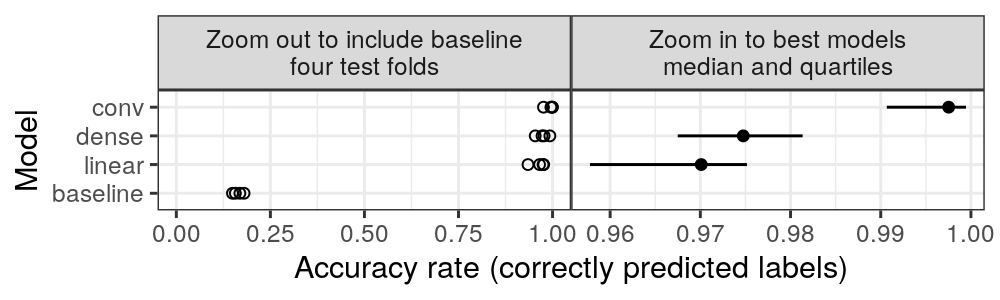
\includegraphics[width=0.8\textwidth]{figure-test-accuracy-both}
  \caption{test accuracy values}
  \label{fig:test-accuracy}
\end{figure}
 
{Accuracy rates for each test fold}
  \begin{itemize}
  \item Always a good idea to compare with the trivial baseline model which always
    predicts the most frequent class in the train set. (ignoring all
    inputs/features) 
  \item Here we see that the baseline is much less accurate than the
    three learned models, so they are clearly learning something non-trivial.
  \item Code for test accuracy figures:
    \url{https://github.com/tdhock/2020-yiqi-summer-school/blob/master/figure-test-accuracy.R}
  \end{itemize}

{Zoom to learned models}
\begin{itemize}
\item Dense neural network slightly more accurate
  than linear model, convoluational significantly more
  accurate than others.
\item Conclusion: convolutional neural network should be preferred
  for most accurate predictions in these data.
\item Maybe not the same conclusion in other data sets, with the
  same models. (always need to do cross-validation experiments to
  see which model is best in any given data set)
\item Maybe other models/algorithms would be even more accurate in
  these data. (more/less layers, more/less units, completely
  different algorithm such as random forests, boosting, etc)
\end{itemize}

\section{Additional reading}

Machine learning is a large field of research with many algorithms,
and there are several useful textbooks that provide overviews from
various perspectives \citep{Bishop2006, Hastie2009, Wasserman2010,
  Murphy2013, Goodfellow2016}.

\paragraph{Reproducibility statement.} Code for figures in this
chapter can be freely downloaded from
\url{https://github.com/tdhock/2020-yiqi-summer-school}

\bibliographystyle{abbrvnat}
\bibliography{refs} 

\end{document}
